\documentclass{article}

\usepackage[brazilian]{babel}

\usepackage{verbatim}
\usepackage{graphicx}
\usepackage{xcolor}

\newcommand{\obs}[1]{\textit{ Obs:#1 }}

\begin{document}
\title{Instalando Arch}
\author{Hashimoto}
\date{}
\maketitle

\section{Preparando Bootloader}\

Primeiro temos que ler o guia de instalação do Arch
\\ (https://wiki.archlinux.org/title/Installation\_guide).
Todos os passos estão descritos lá
(menos os de customização).

Após, temos que baixar a \emph{ISO}
e ``instalar'' num pendrive
(se for fazer em um ``PC de verdade'').
Já que já instalei um arch antes
e vou usar uma VM (\emph{Virtual Machine}),
já tenho a \emph{ISO} e não preciso instalar num pendrive.

\obs{
Se for bootar num PC de verdade lembre-se
de ``spammar'' as \texttt{F-keys} e
ordenar para bootar do pendrive primeiro.
}

\section{Ligando o PC/VM}\

Após ligar, com o pendrive já plugado
vai aparecer a janelinha mágica da sua \emph{ISO}.
Selecione a primeira opção.

\begin{center}
    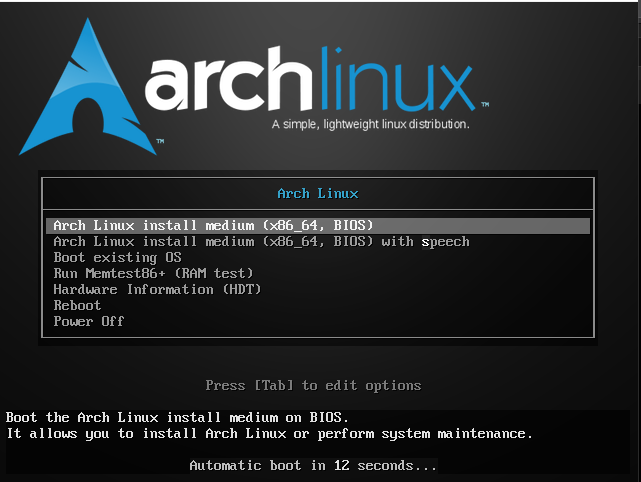
\includegraphics[height=.35\textheight]{Imgs/BootLoader.png}
\end{center}

Vai aparecer um monte de texto escrolando para cima,
aguarde...

\section{Preparando o terreno}\

Se você aguardou, deve estar vendo
uma ``tela preta'' com uma
vaquinha e logo em baixo\\
\texttt{{\color{red}root}@archiso \~{} \#} \\
e um cursorzinho piscando.
Está olhando para um terminal e
não se preocupe, ele não morde.

\begin{center}
    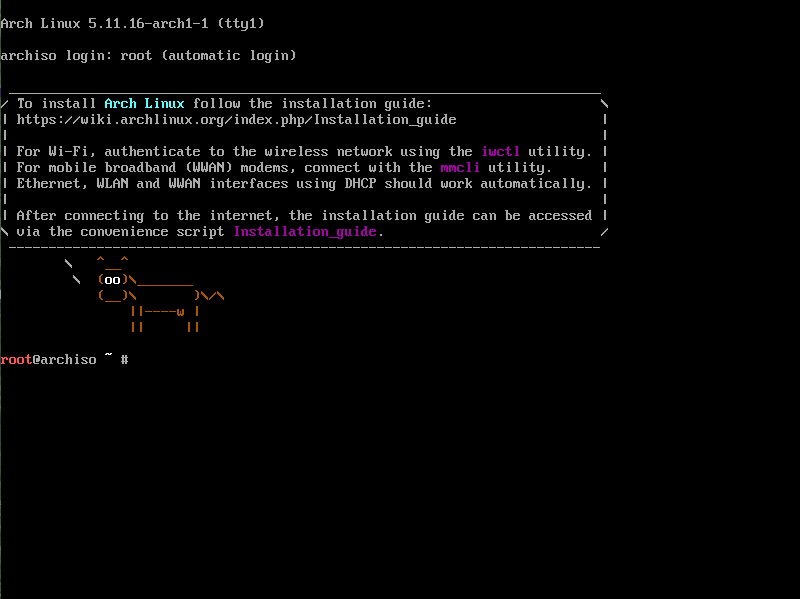
\includegraphics[width=\textwidth]{Imgs/Hello-arch.png}
\end{center}

\obs{
Existe um arquivo no diretório atual chamado
\texttt{install.txt} ele contém o mesmo conteúdo
da Arch Wiki.
Recomendo fortemente que de um \texttt{Alt-2}
para abrir esse txt no seu editor de texto preferido
e usar como guia para o resto da instalação.
Você pode voltar para o outro terminal usando \texttt{Alt-1}.
}

O próximo passo é configurar o seu \emph{layout de teclado}.
O \emph{layout} padrão é Americano.
Se não tem certeza do nome do seu \emph{layout} favorito,
pode procurar usando:

\begin{verbatim}
    # ls /usr/share/kbd/keymaps/**/*.map.gz | less
\end{verbatim}

Eu uso \texttt{br-abnt2}, então usamos:

\begin{verbatim}
    # loadkeys br-abnt2
\end{verbatim}

\obs{
Também dá para trocar a fonte usando \texttt{setfont}.
e as fontes estão em \texttt{/usr/share/kbd/consolefonts}.
}

Fazemos um pequeno teste para saber o modo de boot.
Se o diretório \texttt{/sys/firmware/efi/efivars} existir,
o PC foi bootado com \emph{UEFI},
caso contrário foi bootado com \emph{BIOS} ou \emph{CSM}.

\begin{verbatim}
    # ls /sys/firmware/efi/efivars
    ls: cannot access '/sys/firmware/efi/efivars': No such file or directory
    {2}
\end{verbatim}

Então no meu caso foi com \emph{BIOS} ou \emph{CSM}.

Podemos testar a internet com \texttt{ping -c 3 <seu.dominio.preferido>},
eu gosto do \emph{8.8.8.8}, dá para digitar rapidinho
(o \texttt{-c 3} é para não ter que dar \emph{Ctrl-C} depois).
Como estou em uma VM não preciso fazer muita coisa e já tenho internet.

\begin{center}
    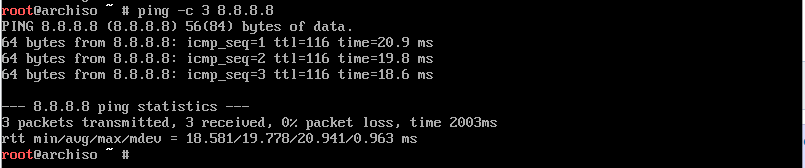
\includegraphics[width=\textwidth]{Imgs/Ping.png}
\end{center}

Vamos usar \texttt{timedatectl set-ntp true}
para ter certeza que o relógio do sistema está certo.

\begin{verbatim}
    --- TL;DR ---
    # loadkeys br-abnt2 --- Configurar o teclado
    # ping -c 3 8.8.8.8 --- Testar se internet funciona
    # timedatectl set-ntp true --- Acertar o relógio do sistema
\end{verbatim}

\section{Particionando o Disco}\

Primeiro temos que achar o nome do/escolher o disco.
Não podemos escolher discos terminados em
\emph{rom}, \emph{loop} ou \emph{airoot}

\begin{verbatim}
    # fdisk -l
\end{verbatim}

\begin{center}
    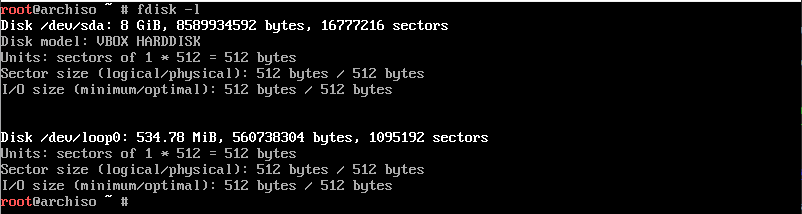
\includegraphics[width=\textwidth]{Imgs/Fdisk-l.png}
\end{center}

Nosso disco é \texttt{/dev/sda/} e tem \emph{8 Gib}. :)

Temos que criar a tabela de partição,
no nosso caso uma \emph{GPT}
\textit{(Por quê, você pergunta? Porque é a opção comum)}.
Vamos usar o próprio \texttt{fdisk} para criar a tabela.

\begin{verbatim}
    # fdisk /dev/sda
\end{verbatim}

\begin{center}
    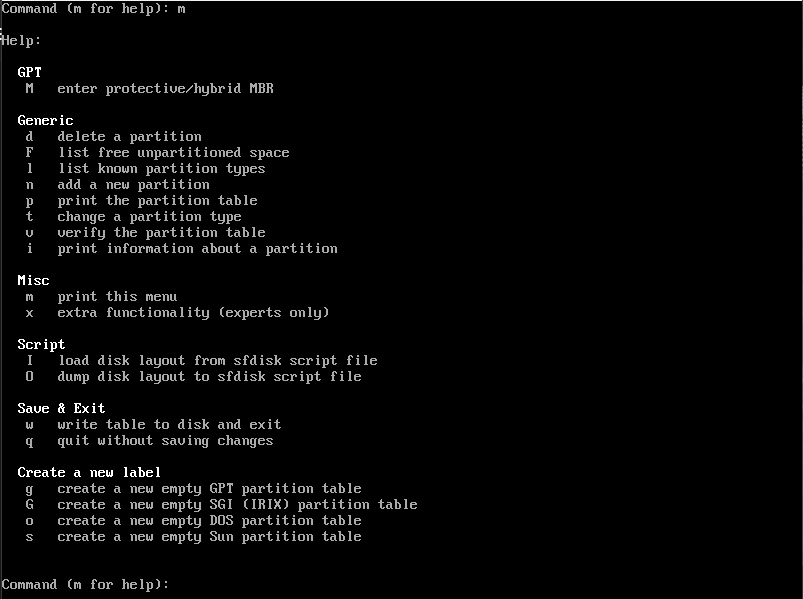
\includegraphics[width=\textwidth]{Imgs/Fdisk-help.png}
\end{center}

Vamos gerar nossa nova tabela com \texttt{g},
criar 3 partições:
uma para \texttt{boot} com \emph{260MiB},
uma para \texttt{/} com \emph{7.2GiB} e
outra para o \texttt{swap} com \emph{512MiB}.

Então nosso input ficou assim (cada \texttt{;} é um \texttt{Enter}):
\begin{verbatim}
    g;n;;+260M;t;4;n;;;+7.2G;n;;;;t;;19;w
\end{verbatim}

Olha que bonita nossa tabela!

\begin{verbatim}
    # fdisk -l /dev/sda
\end{verbatim}

\begin{center}
    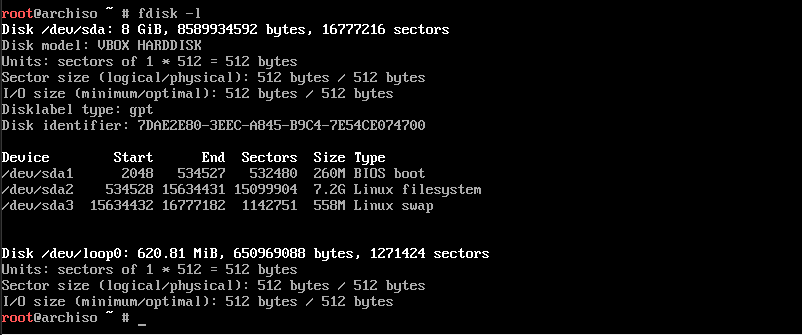
\includegraphics[width=\textwidth]{Imgs/Fdisk-sda.png}
\end{center}

\obs{
Se estivéssemos usando \emph{UEFI}
precisaríamos criar uma partição para boot dela.
}

Agora temos que formartar as partições
e montá-las/ativá-la:

\begin{verbatim}
    --- Formatar ---
    # mkfs.ext4 /dev/sda2
    # mkswap /dev/sda3
    --- Montar ---
    # mount /dev/sda2 /mnt
    --- Ativar ---
    # swapon /dev/sda3
\end{verbatim}

\section{Instalando}\

Os \emph{mirror servers}
(lugares de onde vai ser baixado o sistema)
estão em \texttt{/etc/pacman.d/mirrorlist}.
Podemos trocar a ordem, deletar os mais lentos,
mas a ordem padrão já é boa então vamos só instalar
usando o script:

\begin{verbatim}
    # pacstrap /mnt base linux vim
\end{verbatim}

\obs{
Se não estiver instalando num container ou virtual-machine
passe \texttt{linux-firmware} como um argumento extra.
}

Agora é sentar e esperar...

\section{Configurando o sistema}\

Vamos gerar o \texttt{Fstab}:

\begin{verbatim}
    # genfstab -U /mnt >> /mnt/etc/fstab
\end{verbatim}

Entrar no nosso novo sistema como \emph{root}:

\begin{verbatim}
    # arch-chroot /mnt
\end{verbatim}

Escolher o \emph{Time zone}:

\begin{verbatim}
    # ln -sf /usr/share/zoneinfo/America/Sao_Paulo /etc/localtime
    # hwclock --systohc
\end{verbatim}

Para configurar a localização,
temos que procurar o arquivo \texttt{/etc/locale.gen}
e descomentar a linha com \texttt{pt\_BR.UTF-8 UTF-8}
(para isso que baixamos o \texttt{vim}!).

E depois de descomentar a linha:

\begin{verbatim}
    # locale-gen
    # echo LANG=pt_BR.UTF-8 >> /etc/locale.config
    # echo KEYMAP=br-abnt2 >> /etc/vconsole.config
\end{verbatim}

Configurar o network escolhemos um hostname
e escrevemos em \texttt{/etc/hostname}
e também precisamos escrever em \texttt{/etc/hosts} isso: \\
\begin{verbatim}
    127.0.0.1       localhost
    ::1             localhost
    127.0.1.1       vm-arch.localdomain  vm-arch
\end{verbatim}

\begin{verbatim}
    # echo vm-arch >> /etc/hostname
\end{verbatim}

A última coisa que falta para darmos o primeiro boot
é o boot loader.

\begin{verbatim}
    # pacman -S grub
    # grub-install /dev/sda
    # grub-mkconfig -o /boot/grub/grub.cfg
\end{verbatim}

Antes de dar reboot,
vamos aproveitar o root para escolher
sua senha super-secreta com \texttt{passwd}
e para criar um usuário \emph{shikiyo}:

\begin{verbatim}
    # passwd
    # useradd -m -g users -G whell shikiyo
    # passwd shikiyo
\end{verbatim}

Vamos baixar e configurar utilitários de internet
e também \texttt{sudo},
para o \texttt{sudo} é só
descomentar a linha \texttt{\%wheel ALL=(ALL) ALL}.

\begin{verbatim}
    # pacman -S networkmanager sudo
    # EDITER=vim visudo
    # systemctl enable NetworkManager
\end{verbatim}

Agora vamos dar reboot

\begin{verbatim}
    # exit
    # umount -a
    # reboot
\end{verbatim}

\obs{
Lembrar de retirar o pendrive.
}

\obs{
Agora é um bom momento para clonar a ISO da máquina virtual.
}

\section{Pós-instalando}\

\begin{center}
    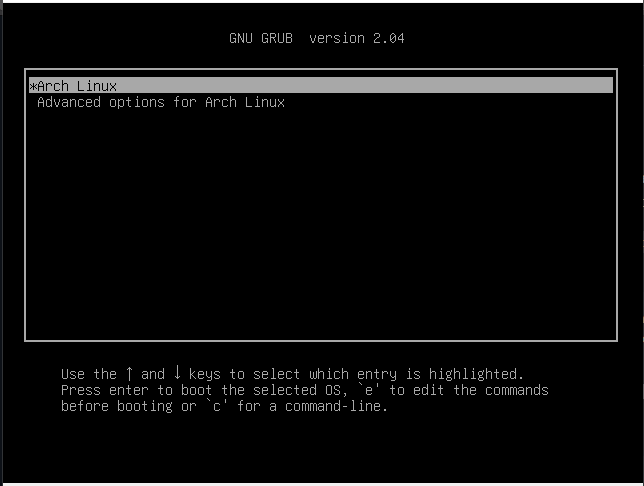
\includegraphics[width=\textwidth]{Imgs/Grub.png}
\end{center}

Esse é o momento de instalar o que seu coração pedir!
Vou instalar apenas o \texttt{xorg} e o \texttt{gnome}.

\begin{verbatim}
    $ sudo pacman -S xorg gnome
    $ sudo systemctl enable gdm
\end{verbatim}

E no próximo reboot teremos uma interface gráfica bonitinha!

\begin{center}
    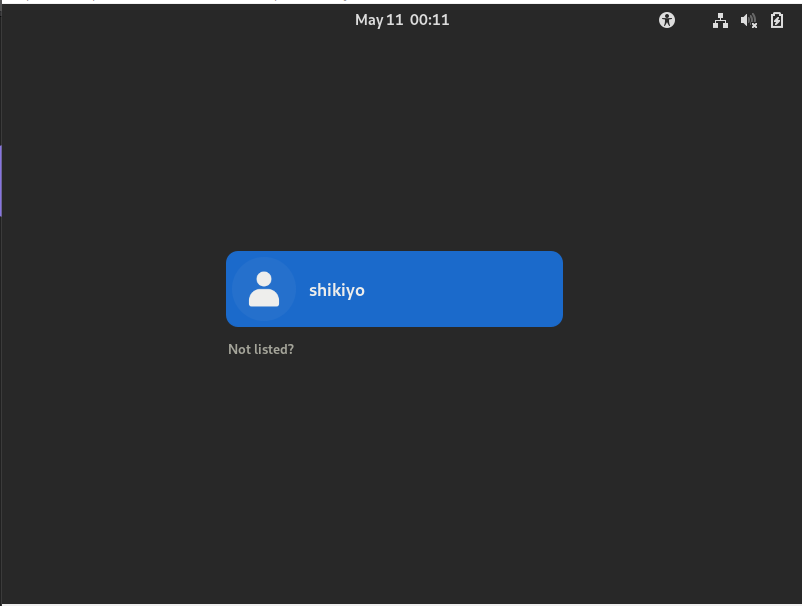
\includegraphics[width=\textwidth]{Imgs/Gnome-1.png}
\end{center}

\begin{center}
    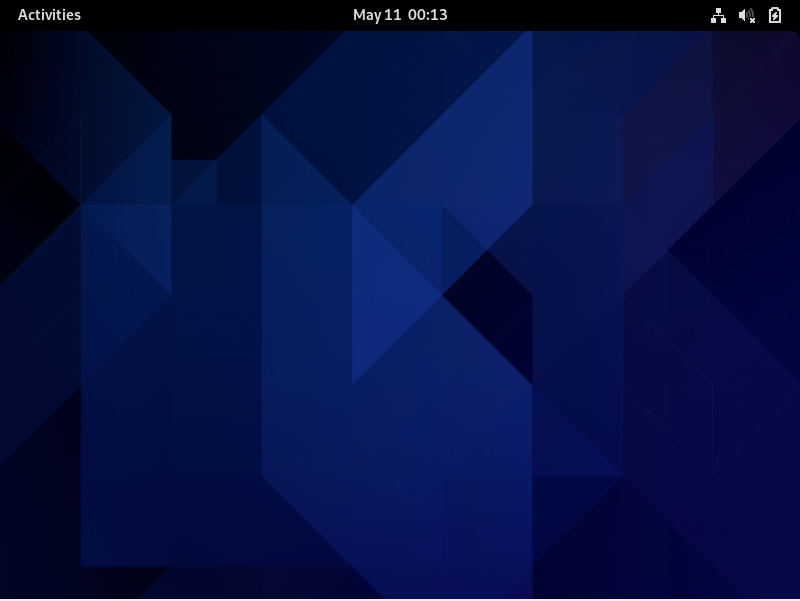
\includegraphics[width=\textwidth]{Imgs/Gnome-2.png}
\end{center}

\end{document}
